\section{Method}
\label{sec:method}
%% Main points:
%% - Preliminary: explain SAM very briefly and how the decoder works
%% - Explain the adapter
%% - How we attach the adapter to the decoder of SAM
%% - Initialization of the adapter
%% - Why we use it in the decoder: less parameters. The encoder should give a good representation already
%% - Image showing everything
We propose a simple, lightweight adapter for the Segment Anything Model (SAM)~\sidecite{sam} that draws inspiration from adaptation techniques in the NLP literature. 

\plainwidefig[t]{1}{Figures/method.pdf}{Illustration of the proposed adaption for SAM Decoder in layer~$\ell$. In each layer, the adaption embeddings are fed along with the dense embeddings to the trainable zero-initialized attention module. Then, the resulting tokens are combined with the decoder embeddings with a trainable gating parameter and a linear MLP.}{fig:method_samda}

\subsection{Segment Anything Model.}
\label{sec:sam}
SAM consists of three primary components: an image encoder, a prompt encoder, and a mask decoder. The image encoder is a standard MAE pre-trained Vision Transformer (ViT)~\sidecite{dosovitskiy2021an} that transforms the input image into an embedding space. The prompt encoder takes either sparse (points, boxes) or dense (masks) annotation formats and produces encoded prompts. Both the image embedding and the encoded prompts are fed to the mask decoder, which consists of a transformer block with a mask prediction head. The transformer block applies two layers of two-way cross-attention operations acting on the image and the prompt embeddings. The result of the transformer is upsampled with an MLP and then fed to a linear classifier, which predicts the final segmentation mask.

\subsection{SAM Decoder Adapter.}
\label{sec:adapter}

The LLaMA-Adapter~\sidecite{llama_adapter} is an adaption method originally introduced to finetune pre-trained LLMs such as LLaMA~\sidecite{llama}. In the context of language generation, this adapter introduces a set of learnable adaption prompts at the higher layers of the LLaMA transformer, and prepends them to the word tokens before the attention operations. 

Our approach brings the idea of prompt-based adaptation from NLP to SAM. We introduce a new learnable adaption prompt~$A_\ell\in\real^{N\times{}D}$ at each layer~$\ell$ of the mask decoder's transformer. The adaptation prompts are used to compute correction factors that modify the embeddings of the transformer without retraining its parameters. Formally, let~$T_\ell\in\real^{M\times D}$ be the embeddings obtained as the output of the cross-attention operation at layer~$\ell$.

We feed $A_\ell$ and~$T_\ell$ to an additional attention block, where the embeddings $T_\ell$ act as queries and the adapter weights~$A_\ell$ act as keys and values\sidenote{We choose to employ the image tokens as queries and the adapter as keys because the image tokens contain important contextual information that should influence the adaptation process. We reinforce this behavior by doing so.},
\begin{eqnarray}
    Q_\ell & = & \linear^q_\ell(T_{\ell}) \in \real^{M\times D_k}, \\
    K_\ell & = & \linear^k_\ell(A_{\ell}) \in \real^{N\times D_k}, \\
    V_\ell & = & \linear^v_\ell(A_{\ell}) \in \real^{N\times D_v}.
\end{eqnarray}
The attention scores are calculated as usual,
\begin{equation}
    S_\ell = \softmax\left(\dfrac{Q_\ell{}K_\ell^T}{\sqrt{D_v}}\right)V_\ell \in \real^{M\times D_v},
\end{equation}
and projected back to the model dimension~$D$ with a linear layer, $S'_\ell=\linear^o_\ell(S_\ell)$. The result~$S'_\ell$ serves as the correction factor of the original embeddings,
\begin{equation}
    T'_\ell = \linear^t_\ell(T_\ell + g_\ell \cdot S'_\ell),
\end{equation}
where the learnable gating factor~$g_\ell\in\real$ is initialized to~0 to ensure no disruption during the early stages of adaptation learning. The entire procedure is summarized in \cref{fig:method_samda,fig:neural_diagram}\sidenote{\cref{fig:neural_diagram} has been created following~\cite{abbott2024neural}, a work that proposes a new standard for neural diagram representation.}.

\begin{figure}[t]
    \centering
    \resizebox{\columnwidth}{!}{%
            
\tikzset{every picture/.style={line width=0.9pt}} %set default line width to 0.75pt        

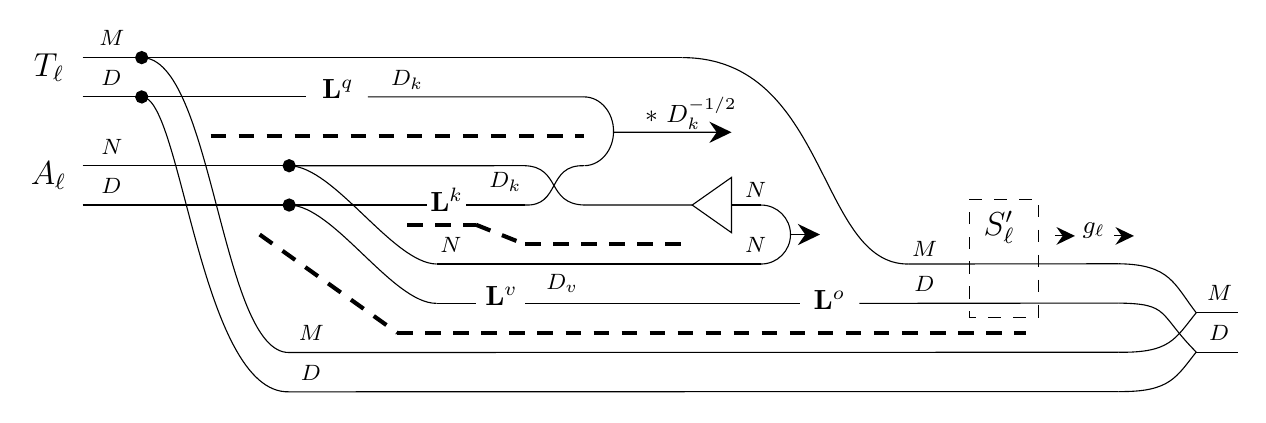
\begin{tikzpicture}[x=0.75pt,y=0.75pt,yscale=-1,xscale=1]
%uncomment if require: \path (0,209); %set diagram left start at 0, and has height of 209

%Straight Lines [id:da9318541924872752] 
\draw [color={rgb, 255:red, 0; green, 0; blue, 0 }  ,draw opacity=1 ]   (28.52,24.09) -- (317.42,24.09) ;
%Straight Lines [id:da9479457685518922] 
\draw [color={rgb, 255:red, 0; green, 0; blue, 0 }  ,draw opacity=1 ]   (284.27,60.08) -- (338.1,60.07) ;
\draw [shift={(341.1,60.07)}, rotate = 179.99] [fill={rgb, 255:red, 0; green, 0; blue, 0 }  ,fill opacity=1 ][line width=0.08]  [draw opacity=0] (10.72,-5.15) -- (0,0) -- (10.72,5.15) -- (7.12,0) -- cycle    ;
%Straight Lines [id:da9416679881824883] 
\draw [color={rgb, 255:red, 0; green, 0; blue, 0 }  ,draw opacity=1 ]   (28.52,43.04) -- (136.25,43.04) ;
%Straight Lines [id:da820033648196937] 
\draw [color={rgb, 255:red, 0; green, 0; blue, 0 }  ,draw opacity=1 ]   (28.52,76.19) -- (127.98,76.19) ;
%Straight Lines [id:da3464705312194676] 
\draw [color={rgb, 255:red, 0; green, 0; blue, 0 }  ,draw opacity=1 ]   (28.52,95.13) -- (127.98,95.13) ;
%Straight Lines [id:da6907623082124388] 
\draw [color={rgb, 255:red, 0; green, 0; blue, 0 }  ,draw opacity=1 ][line width=1.5]  [dash pattern={on 5.63pt off 4.5pt}]  (90.09,61.98) -- (270.06,61.98) ;
%Straight Lines [id:da2178356496804179] 
\draw [color={rgb, 255:red, 0; green, 0; blue, 0 }  ,draw opacity=1 ]   (199.02,123.55) -- (355.31,123.55) ;
%Shape: Arc [id:dp9189314153891996] 
\draw  [draw opacity=0] (270.28,76.17) .. controls (278.02,76.03) and (284.27,68.67) .. (284.27,59.6) .. controls (284.27,50.44) and (277.91,43.02) .. (270.06,43.02) .. controls (270.04,43.02) and (270.01,43.02) .. (269.99,43.02) -- (270.06,59.6) -- cycle ; \draw  [color={rgb, 255:red, 0; green, 0; blue, 0 }  ,draw opacity=1 ] (270.28,76.17) .. controls (278.02,76.03) and (284.27,68.67) .. (284.27,59.6) .. controls (284.27,50.44) and (277.91,43.02) .. (270.06,43.02) .. controls (270.04,43.02) and (270.01,43.02) .. (269.99,43.02) ;  
%Curve Lines [id:da9542147110842154] 
\draw [color={rgb, 255:red, 0; green, 0; blue, 0 }  ,draw opacity=1 ]   (241.64,76.17) .. controls (258.95,76.9) and (252,94.58) .. (270.06,95.12) ;
%Curve Lines [id:da811837651150005] 
\draw [color={rgb, 255:red, 0; green, 0; blue, 0 }  ,draw opacity=1 ]   (241.64,95.12) .. controls (258.95,95.84) and (252,75.63) .. (270.06,76.17) ;
%Straight Lines [id:da9225972703365359] 
\draw [color={rgb, 255:red, 0; green, 0; blue, 0 }  ,draw opacity=1 ]   (270.06,95.12) -- (322.16,95.13) ;
%Shape: Arc [id:dp012632027617723418] 
\draw  [draw opacity=0] (355.31,123.55) .. controls (363.16,123.55) and (369.52,117.19) .. (369.52,109.34) .. controls (369.52,101.5) and (363.16,95.13) .. (355.31,95.13) -- (355.31,109.34) -- cycle ; \draw  [color={rgb, 255:red, 0; green, 0; blue, 0 }  ,draw opacity=1 ] (355.31,123.55) .. controls (363.16,123.55) and (369.52,117.19) .. (369.52,109.34) .. controls (369.52,101.5) and (363.16,95.13) .. (355.31,95.13) ;  
%Straight Lines [id:da8996757312086063] 
\draw [color={rgb, 255:red, 0; green, 0; blue, 0 }  ,draw opacity=1 ]   (341.1,95.13) -- (355.31,95.13) ;
%Shape: Triangle [id:dp9355169581622589] 
\draw   (322.16,95.13) -- (341.1,81.81) -- (341.1,108.45) -- cycle ;
%Straight Lines [id:da9948364456698844] 
\draw [color={rgb, 255:red, 0; green, 0; blue, 0 }  ,draw opacity=1 ]   (369.52,109.34) -- (380.73,109.34) ;
\draw [shift={(383.73,109.34)}, rotate = 180] [fill={rgb, 255:red, 0; green, 0; blue, 0 }  ,fill opacity=1 ][line width=0.08]  [draw opacity=0] (10.72,-5.15) -- (0,0) -- (10.72,5.15) -- (7.12,0) -- cycle    ;
%Straight Lines [id:da6043160547682214] 
\draw [color={rgb, 255:red, 0; green, 0; blue, 0 }  ,draw opacity=1 ]   (426.35,123.55) -- (527.64,123.42) ;
%Curve Lines [id:da6867804311377057] 
\draw [color={rgb, 255:red, 0; green, 0; blue, 0 }  ,draw opacity=1 ]   (317.42,24.09) .. controls (387.99,24.27) and (382.54,123.97) .. (426.35,123.55) ;
%Curve Lines [id:da35185424855257263] 
\draw [color={rgb, 255:red, 0; green, 0; blue, 0 }  ,draw opacity=1 ]   (127.98,76.19) .. controls (149.75,76.35) and (177.86,123.17) .. (199.02,123.55) ;
\draw [shift={(127.98,76.19)}, rotate = 0.42] [color={rgb, 255:red, 0; green, 0; blue, 0 }  ,draw opacity=1 ][fill={rgb, 255:red, 0; green, 0; blue, 0 }  ,fill opacity=1 ][line width=0.75]      (0, 0) circle [x radius= 2.68, y radius= 2.68]   ;
%Straight Lines [id:da1325813172340935] 
\draw [color={rgb, 255:red, 0; green, 0; blue, 0 }  ,draw opacity=1 ][line width=1.5]  [dash pattern={on 5.63pt off 4.5pt}]  (241.64,114.08) -- (322.16,114.08) ;
%Curve Lines [id:da1474512418867049] 
\draw [color={rgb, 255:red, 0; green, 0; blue, 0 }  ,draw opacity=1 ]   (127.98,95.13) .. controls (149.51,95.3) and (177.86,142.66) .. (199.02,142.5) ;
\draw [shift={(127.98,95.13)}, rotate = 0.43] [color={rgb, 255:red, 0; green, 0; blue, 0 }  ,draw opacity=1 ][fill={rgb, 255:red, 0; green, 0; blue, 0 }  ,fill opacity=1 ][line width=0.75]      (0, 0) circle [x radius= 2.68, y radius= 2.68]   ;
%Straight Lines [id:da0024795885398030126] 
\draw [color={rgb, 255:red, 0; green, 0; blue, 0 }  ,draw opacity=1 ]   (165.87,43.04) -- (269.99,43.02) ;
%Straight Lines [id:da5129391997953758] 
\draw [color={rgb, 255:red, 0; green, 0; blue, 0 }  ,draw opacity=1 ]   (213.23,95.13) -- (241.64,95.13) ;
%Straight Lines [id:da5222565283453322] 
\draw [color={rgb, 255:red, 0; green, 0; blue, 0 }  ,draw opacity=1 ]   (199.02,142.5) -- (217.96,142.5) ;
%Straight Lines [id:da5713516733511401] 
\draw [color={rgb, 255:red, 0; green, 0; blue, 0 }  ,draw opacity=1 ]   (241.64,142.5) -- (374.25,142.5) ;
%Straight Lines [id:da7381871923413768] 
\draw [color={rgb, 255:red, 0; green, 0; blue, 0 }  ,draw opacity=1 ][line width=1.5]  [dash pattern={on 5.63pt off 4.5pt}]  (184.81,104.61) -- (217.96,104.61) ;
%Straight Lines [id:da4800244787455168] 
\draw [color={rgb, 255:red, 0; green, 0; blue, 0 }  ,draw opacity=1 ][line width=1.5]  [dash pattern={on 5.63pt off 4.5pt}]  (217.96,104.61) -- (241.64,114.08) ;
%Straight Lines [id:da3222725473972332] 
\draw [color={rgb, 255:red, 0; green, 0; blue, 0 }  ,draw opacity=1 ]   (402.67,142.5) -- (527.64,142.37) ;
%Shape: Rectangle [id:dp5331533235436763] 
\draw  [dash pattern={on 4.5pt off 4.5pt}] (455.71,92.29) -- (488.87,92.29) -- (488.87,149.13) -- (455.71,149.13) -- cycle ;
%Curve Lines [id:da5832391229104559] 
\draw [color={rgb, 255:red, 0; green, 0; blue, 0 }  ,draw opacity=1 ]   (56.94,43.04) .. controls (76.07,42.2) and (85.17,186.36) .. (127.98,185.12) ;
\draw [shift={(56.94,43.04)}, rotate = 357.48] [color={rgb, 255:red, 0; green, 0; blue, 0 }  ,draw opacity=1 ][fill={rgb, 255:red, 0; green, 0; blue, 0 }  ,fill opacity=1 ][line width=0.75]      (0, 0) circle [x radius= 2.68, y radius= 2.68]   ;
%Curve Lines [id:da07594588484193321] 
\draw [color={rgb, 255:red, 0; green, 0; blue, 0 }  ,draw opacity=1 ]   (56.94,24.09) .. controls (91.23,24.01) and (95.02,166.66) .. (127.98,166.18) ;
\draw [shift={(56.94,24.09)}, rotate = 359.86] [color={rgb, 255:red, 0; green, 0; blue, 0 }  ,draw opacity=1 ][fill={rgb, 255:red, 0; green, 0; blue, 0 }  ,fill opacity=1 ][line width=0.75]      (0, 0) circle [x radius= 2.68, y radius= 2.68]   ;
%Straight Lines [id:da4069702799953998] 
\draw [color={rgb, 255:red, 0; green, 0; blue, 0 }  ,draw opacity=1 ]   (127.98,166.18) -- (527.64,166.05) ;
%Straight Lines [id:da04501569766126101] 
\draw [color={rgb, 255:red, 0; green, 0; blue, 0 }  ,draw opacity=1 ]   (127.98,185.12) -- (527.64,184.99) ;
%Straight Lines [id:da10656219889721918] 
\draw [color={rgb, 255:red, 0; green, 0; blue, 0 }  ,draw opacity=1 ]   (525.53,110) -- (532,110) ;
\draw [shift={(535,110)}, rotate = 180] [fill={rgb, 255:red, 0; green, 0; blue, 0 }  ,fill opacity=1 ][line width=0.08]  [draw opacity=0] (8.93,-4.29) -- (0,0) -- (8.93,4.29) -- (5.93,0) -- cycle    ;
%Straight Lines [id:da8097902856805503] 
\draw [color={rgb, 255:red, 0; green, 0; blue, 0 }  ,draw opacity=1 ]   (497.11,110) -- (503.58,110) ;
\draw [shift={(506.58,110)}, rotate = 180] [fill={rgb, 255:red, 0; green, 0; blue, 0 }  ,fill opacity=1 ][line width=0.08]  [draw opacity=0] (8.93,-4.29) -- (0,0) -- (8.93,4.29) -- (5.93,0) -- cycle    ;
%Curve Lines [id:da8240921966457793] 
\draw [color={rgb, 255:red, 0; green, 0; blue, 0 }  ,draw opacity=1 ]   (527.64,123.42) .. controls (552.56,123.76) and (554.33,133.2) .. (565,147.02) ;
%Curve Lines [id:da8752997693066615] 
\draw [color={rgb, 255:red, 0; green, 0; blue, 0 }  ,draw opacity=1 ]   (527.64,166.05) .. controls (552.56,166.38) and (554.78,159.65) .. (565,147.02) ;
%Curve Lines [id:da10181116987059924] 
\draw [color={rgb, 255:red, 0; green, 0; blue, 0 }  ,draw opacity=1 ]   (527.64,142.37) .. controls (552.56,142.7) and (546.42,147.31) .. (565,165.97) ;
%Curve Lines [id:da853323633730164] 
\draw [color={rgb, 255:red, 0; green, 0; blue, 0 }  ,draw opacity=1 ]   (527.64,184.99) .. controls (552.56,185.32) and (555.44,177.87) .. (565,165.97) ;
%Straight Lines [id:da546971982487424] 
\draw    (565,147.02) -- (585,147.02) ;
%Straight Lines [id:da31488236797131886] 
\draw    (565,165.97) -- (585,165.97) ;
%Straight Lines [id:da615457324230881] 
\draw [color={rgb, 255:red, 0; green, 0; blue, 0 }  ,draw opacity=1 ][line width=1.5]  [dash pattern={on 5.63pt off 4.5pt}]  (180.08,156.7) -- (483.18,156.7) ;
%Straight Lines [id:da1734793752436845] 
\draw [color={rgb, 255:red, 0; green, 0; blue, 0 }  ,draw opacity=1 ]   (127.98,95.13) -- (194.28,95.13) ;
%Straight Lines [id:da411491139550342] 
\draw [color={rgb, 255:red, 0; green, 0; blue, 0 }  ,draw opacity=1 ]   (127.98,76.19) -- (241.64,76.17) ;
%Straight Lines [id:da36908543265196636] 
\draw [color={rgb, 255:red, 0; green, 0; blue, 0 }  ,draw opacity=1 ][line width=1.5]  [dash pattern={on 5.63pt off 4.5pt}]  (113.77,109.34) -- (180.08,156.7) ;

% Text Node
\draw (35.23,9.94) node [anchor=north west][inner sep=0.75pt]  [font=\fontsize{0.82em}{0.99em}\selectfont]  {$M$};
% Text Node
\draw (3.76,21.05) node [anchor=north west][inner sep=0.75pt]  [font=\large]  {$T_{\ell }$};
% Text Node
\draw (36.23,28.89) node [anchor=north west][inner sep=0.75pt]  [font=\fontsize{0.82em}{0.99em}\selectfont]  {$D$};
% Text Node
\draw (2.26,73.14) node [anchor=north west][inner sep=0.75pt]  [font=\large]  {$A_{\ell }$};
% Text Node
\draw (36.23,80.98) node [anchor=north west][inner sep=0.75pt]  [font=\fontsize{0.82em}{0.99em}\selectfont]  {$D$};
% Text Node
\draw (36.23,62.04) node [anchor=north west][inner sep=0.75pt]  [font=\fontsize{0.82em}{0.99em}\selectfont]  {$N$};
% Text Node
\draw (298.21,41.97) node [anchor=north west][inner sep=0.75pt]  [font=\small]  {$*\ D_{k}^{-1/2}$};
% Text Node
\draw (142.61,33.5) node [anchor=north west][inner sep=0.75pt]  [font=\normalsize]  {$\mathbf{L}^{q}$};
% Text Node
\draw (175.79,28.86) node [anchor=north west][inner sep=0.75pt]  [font=\fontsize{0.82em}{0.99em}\selectfont]  {$D_{k}$};
% Text Node
\draw (194.7,85.59) node [anchor=north west][inner sep=0.75pt]  [font=\normalsize]  {$\mathbf{L}^{k}$};
% Text Node
\draw (223.15,78.12) node [anchor=north west][inner sep=0.75pt]  [font=\fontsize{0.82em}{0.99em}\selectfont]  {$D_{k}$};
% Text Node
\draw (221.22,132.95) node [anchor=north west][inner sep=0.75pt]  [font=\normalsize]  {$\mathbf{L}^{v}$};
% Text Node
\draw (250.61,127.37) node [anchor=north west][inner sep=0.75pt]  [font=\fontsize{0.82em}{0.99em}\selectfont]  {$D_{v}$};
% Text Node
\draw (199.62,109.4) node [anchor=north west][inner sep=0.75pt]  [font=\fontsize{0.82em}{0.99em}\selectfont]  {$N$};
% Text Node
\draw (346.44,82.88) node [anchor=north west][inner sep=0.75pt]  [font=\fontsize{0.82em}{0.99em}\selectfont]  {$N$};
% Text Node
\draw (346.44,109.4) node [anchor=north west][inner sep=0.75pt]  [font=\fontsize{0.82em}{0.99em}\selectfont]  {$N$};
% Text Node
\draw (461.29,96.82) node [anchor=north west][inner sep=0.75pt]  [font=\large]  {$S'_{\ell }$};
% Text Node
\draw (379.41,134.85) node [anchor=north west][inner sep=0.75pt]  [font=\normalsize]  {$\mathbf{L}^{o}$};
% Text Node
\draw (426.9,111.29) node [anchor=north west][inner sep=0.75pt]  [font=\fontsize{0.82em}{0.99em}\selectfont]  {$M$};
% Text Node
\draw (427.9,128.34) node [anchor=north west][inner sep=0.75pt]  [font=\fontsize{0.82em}{0.99em}\selectfont]  {$D$};
% Text Node
\draw (509,102.4) node [anchor=north west][inner sep=0.75pt]  [font=\small]  {$g_{\ell }$};
% Text Node
\draw (569,132.4) node [anchor=north west][inner sep=0.75pt]  [font=\fontsize{0.82em}{0.99em}\selectfont]  {$M$};
% Text Node
\draw (570,151.82) node [anchor=north west][inner sep=0.75pt]  [font=\fontsize{0.82em}{0.99em}\selectfont]  {$D$};
% Text Node
\draw (131.37,152.02) node [anchor=north west][inner sep=0.75pt]  [font=\fontsize{0.82em}{0.99em}\selectfont]  {$M$};
% Text Node
\draw (132.37,170.97) node [anchor=north west][inner sep=0.75pt]  [font=\fontsize{0.82em}{0.99em}\selectfont]  {$D$};
\end{tikzpicture}
}
\sidecaption{Neural circuit diagram for the proposed SAM-Decoder-Adapter following the methodology described in~\cite{abbott2024neural}.\label{fig:neural_diagram}
}
\end{figure}

We note that this approach could potentially be implemented within the model's encoder. However, we deliberately decided not to pursue this route for two main reasons: (1) the image representation generated by the encoder is already high-quality due to a pre-trained model on similar data, and (2) any modifications to the encoder's parameters may necessitate retraining of the mask decoder as well. Given our objective of reducing the number of parameters, we confine the implementation solely to the decoder. In \Cref{sec:ablation_samda}, we show experimentally how the location of the adapter affects the model's performance.
